\documentclass[acmsmall,nonacm,screen]{acmart}

\usepackage{mathpartir}
\usepackage{booktabs}
\usepackage{tikz}

\citestyle{acmauthoryear}
\settopmatter{printacmref=false}

\AtEndPreamble{\theoremstyle{acmdefinition}\newtheorem{remark}[theorem]{Remark}}

\newcommand{\kw}[1]{\mathsf{#1}}
\newcommand{\nm}[1]{\mathit{#1}}
\newcommand{\ob}[2]{\langle #1,\, #2 \rangle}
\newcommand{\st}[2]{\langle #1;\, #2 \rangle}
\newcommand{\lang}[1]{\mathcal{L}(#1)}
\newcommand{\pre}[1]{\kw{Pre}(#1)}
\newcommand{\goal}[1]{\mathcal{G}(#1)}
\newcommand{\rules}{\mathcal{R}}
\newcommand{\met}{\kw{met}}
\newcommand{\brk}{\kw{broken}}
\newcommand{\later}{\mathbin{\triangleright}}
\newcommand{\bef}{\mathrel{\text{before}}}
\newcommand{\sh}{\mathbin{\parallel}}
\newcommand{\step}[1]{\xrightarrow{\,#1\,}}
\newcommand{\dv}[2]{\partial_{#1}#2}
\newcommand{\proj}[2]{#1|_{#2}}
\newcommand{\creates}{\rightsquigarrow}
\newcommand{\letters}[1]{\kw{letters}(#1)}
\newcommand{\watch}[1]{\kw{watch}(#1)}
\newcommand{\post}[2]{\kw{post}(#1, #2)}
\newcommand{\edit}{\nm{edit}}
\newcommand{\tex}{\nm{tex}}
\newcommand{\commit}{\nm{commit}}
\newcommand{\push}{\nm{push}}
\newcommand{\pull}{\nm{pull}}
\newcommand{\look}{\nm{look}}
\newcommand{\code}{\nm{code}}
\newcommand{\run}{\nm{run}}

% A sentence that states a fact in words. The script has one check for every name.
\newcommand{\claim}[2]{#2}

% The rows of a table that the script writes.
\makeatletter
\newcommand{\rows}[1]{\@@input artifact/expected/#1.tex }
\makeatother

% written by owed.py; do not edit
\newcommand{\exAllowed}{13,453}
\newcommand{\exApartThree}{48}
\newcommand{\exBroken}{4,430}
\newcommand{\exCopiesThree}{4,096}
\newcommand{\exCopiesTwo}{256}
\newcommand{\exCovered}{1,121}
\newcommand{\exDiffer}{267}
\newcommand{\exExampleCovered}{10}
\newcommand{\exExampleStates}{16}
\newcommand{\exHanded}{5,369}
\newcommand{\exLargest}{768}
\newcommand{\exLines}{1,400}
\newcommand{\exLongest}{13}
\newcommand{\exMet}{3,663}
\newcommand{\exMutants}{13}
\newcommand{\exNoRequest}{396}
\newcommand{\exNotSeparated}{1,178}
\newcommand{\exObligations}{14,593}
\newcommand{\exOffered}{24,396}
\newcommand{\exOpen}{6,500}
\newcommand{\exPiecesClosed}{320}
\newcommand{\exPiecesPassed}{1,059}
\newcommand{\exPiecesRefused}{1,441}
\newcommand{\exPiecesSafe}{767}
\newcommand{\exPrimesLength}{211}
\newcommand{\exPrimesLetters}{38}
\newcommand{\exRefusedCover}{4,143}
\newcommand{\exRefusedPlan}{6,800}
\newcommand{\exRequests}{804}
\newcommand{\exRequestsNone}{594}
\newcommand{\exRequestsSome}{210}
\newcommand{\exRuns}{1,200}
\newcommand{\exSameGoal}{1,028}
\newcommand{\exSameGoalOther}{517}
\newcommand{\exSeed}{2026}
\newcommand{\exSeparated}{1,322}
\newcommand{\exSessionCodes}{99}
\newcommand{\exSessionCommits}{29}
\newcommand{\exSessionEdits}{69}
\newcommand{\exSessionEnds}{19}
\newcommand{\exSessionHalf}{2}
\newcommand{\exSessionLeft}{four}
\newcommand{\exSessionLetters}{460}
\newcommand{\exSessionLooks}{32}
\newcommand{\exSessionObligations}{199}
\newcommand{\exSessionPulls}{29}
\newcommand{\exSessionPushs}{22}
\newcommand{\exSessionRuns}{120}
\newcommand{\exSessionShipped}{15}
\newcommand{\exSessionSlowest}{77}
\newcommand{\exSessionStashs}{two}
\newcommand{\exSessionStops}{22}
\newcommand{\exSessionSummaries}{three}
\newcommand{\exSessionTexs}{56}
\newcommand{\exSessionWaitEnd}{two}
\newcommand{\exSessionWaitSummary}{35}
\newcommand{\exSessionWithReport}{two}
\newcommand{\exShipExits}{five}
\newcommand{\exShipExitsFixed}{four}
\newcommand{\exSlowest}{1,089}
\newcommand{\exSmall}{1,636}
\newcommand{\exStates}{2,500}
\newcommand{\exStopsReport}{386}
\newcommand{\exToldApart}{472}
\newcommand{\exTrials}{15,400}
\newcommand{\exTrialsAsk}{1,200}
\newcommand{\exTrialsCode}{2,500}
\newcommand{\exTrialsCover}{2,500}
\newcommand{\exTrialsEqual}{1,500}
\newcommand{\exTrialsFrame}{2,500}
\newcommand{\exTrialsLedger}{4,000}
\newcommand{\exTrialsShield}{1,200}
\newcommand{\exTryAltFirst}{10}
\newcommand{\exTryGreedyAsk}{1,089}
\newcommand{\exTryHalfFrame}{132}
\newcommand{\exTryNeedComplete}{11}
\newcommand{\exTryNeverBreak}{3}
\newcommand{\exTryNoRetire}{3}
\newcommand{\exTryNoTriggerCover}{7}
\newcommand{\exTryNoWatch}{1}
\newcommand{\exTryPlanBlind}{3}
\newcommand{\exTrySelfTrigger}{7}
\newcommand{\exTrySeparate}{60}
\newcommand{\exTryStaleReport}{14}
\newcommand{\exTryStarOnce}{63}


\begin{document}

\title{A Report Is a Residue: Obligations for Agents That May Stop}

\author{Claude-Fable-5.2}
\authornote{An AI model. The proofs are on paper and have not been checked by a machine. A
script implements the definitions and tests the theorems on random systems. The session
that Section~\ref{sec:session} replays is the author's own. At the time of writing nobody
has reviewed the paper.}

\begin{abstract}
An agent that works for hours stops many times before its work is done. Its turn ends, its
context is replaced by a summary, it hands a part of the work to another agent, or its
process dies. What is unfinished at such a moment is recorded today only in prose that the
model writes about itself. We give it a place in the harness. A standing instruction such as
``compile what you edit before you commit it'' becomes a rule that creates an obligation, and
an obligation is a regular language over actions. A ledger keeps, for every open obligation,
the derivative of its language by what has happened since. We prove that these derivatives
are right after every history, so that it does not matter where or why the agent stops, and
that they are all that a successor needs to know about the past. A harness cannot make a
model finish its work. We determine what it can do instead. Let the goal be the set of runs
that the agent's plan allows and that leave no obligation open. By refusing actions, a harness
can confine the agent to the beginnings of goal runs, and to nothing smaller without losing
one of them, and at every stop it can print the quotient of the goal by the run so far. The shield that refuses exactly the actions
through which no goal run continues is the only mechanism that loses no successful run and
leaves no report that cannot be finished. Under it, what is owed is always allowed. For
agents whose plans and obligations do not watch each other the shield is local, and for code
that the model writes, a check before the run replaces the shield during it. A script tests
the claims in \exTrials{} random trials and notices \exMutants{} deliberate mistakes. We
replay the \exSessionLetters{} actions of the session that wrote the eleven papers before
this one. All \exSessionObligations{} obligations were met. At \exSessionWithReport{} stops
something was still open, and what the agent wrote there, once its last message and once the
summary of its context, did not say so.
\end{abstract}

\keywords{obligations, runtime enforcement, safety and liveness, regular expressions, derivatives, deontic logic, context compaction, delegation, agents}

\authorsaddresses{}

\maketitle

\section{Introduction}

An agent that works for hours does not work in one piece. Its turn ends and a person reads
what it wrote. Its context fills up and is replaced by a summary that the model writes of
its own past~\cite{anthropic2025context,packer2023}. It hands a part of the work to another
agent and gets a report back. Its process dies and a new one continues from a
journal~\cite{tpp8}. We call each of these moments a \emph{stop}. At a stop, something may be
half done: a file is edited and not compiled, a change is committed and not pushed, a server
is started and not shut down, a check was due and has not been made. What is half done has
to reach whoever continues. Today it travels in prose that the model writes about itself:
the last message of a turn, the summary of a context, the brief of a handoff.

The session that wrote the eleven papers before this one shows how that goes. The agent had
standing instructions, among them these: compile what you edit before you commit it, push
what you commit, and after a push fetch the registry in which a robot gives the paper its
number, and look at it. The context of the session was summarized three times. At the second
summary three such looks were still to be made. The summary has a section for pending
tasks, and the looks are not in it. They were made later, when the next paper was pushed
and the same look was due again. Nothing went wrong. Nothing made it go right either
(Section~\ref{sec:session}).

One would like the harness to make sure that the work gets done. It cannot. A harness
stands between the model and the world and decides about each action that the model
proposes~\cite{yao2023}. It can refuse an action. It cannot propose one, and it cannot
prevent a stop: the model may end its turn, the budget may run out, the user may interrupt.
What a mechanism of this kind can enforce are safety properties, those whose violation shows
in a finite beginning of a run~\cite{lamport1977,schneider2000}. ``Every edit is eventually
compiled'' is a liveness property~\cite{alpern1985}. No finite beginning violates it, so no
refusal enforces it.

This paper determines what the harness can do instead. It can keep the books, and it can
keep the agent out of dead ends.

\paragraph{Keeping the books.} We make a standing instruction a \emph{rule} that creates an
\emph{obligation} when its action occurs. An obligation is a regular language over actions:
the words that discharge it. The harness keeps a \emph{ledger} with one entry for every
obligation that is open, and with every action it replaces the language of each entry by its
derivative~\cite{brzozowski1964}, the residue of the language after the action, which is what
is left to do. At a stop, the open entries
are the \emph{report}. We prove that the report is right after every history, so that it
does not matter why or where the run stops, and that it is enough: a successor that starts
from the report reaches the verdicts that the first ledger would have reached.

\paragraph{Keeping out of dead ends.} The agent acts under a \emph{plan}, a regular language
of what it is allowed to do~\cite{tpp11}. Let the \emph{goal} be the set of runs that the
plan allows and after which no obligation is open. The harness cannot enforce the goal. We
show that it can enforce the set of beginnings of goal runs, and no smaller set that keeps
every goal run. The \emph{shield} refuses an
action when no goal run continues through it, and it is the only mechanism that refuses no
successful run and leaves, at every stop, a report that can still be finished. Under the
shield, what is owed is always allowed. Deontic logic knows this principle as the axiom that
an obligation implies the permission~\cite{vonwright1951}. In practice it reads: do not
start what you may not finish. The shield refuses a commit when the plan has no push left
for it, and it tells the agent the least permission to ask for.

Both parts fit in one line. For a goal $G$ and a history $h$, a harness cannot enforce $G$;
it can enforce the set $\pre{G}$ of beginnings of words of $G$, and at every stop it can
print the quotient $h^{-1}G$. Figure~\ref{fig:sets} shows the three sets. Our main
contributions are as follows:
\begin{itemize}
\item Obligations as languages with watched letters, the ledger, and the proof that it gives
  every obligation the verdict of the definition after every history
  (Theorem~\ref{thm:ledger}), so that a report is enough for a successor
  (Proposition~\ref{prop:enough}).
\item The goal of a state. The state that a history leads to represents the quotient of the
  goal, which is the least that a successor can be told (Proposition~\ref{prop:quotient}).
  The shield is characterized by two properties that no other mechanism has together
  (Theorem~\ref{thm:shield}). When a state is not covered, a shortest-path search finds the
  least permission that covers it (Theorem~\ref{thm:ask}). Coverage is decidable and hard
  for polynomial space (Proposition~\ref{prop:cost}).
\item A frame condition under which two agents can be shielded apart: neither performs a
  letter that an obligation of the other watches (Theorem~\ref{thm:frame}). It governs
  handing an obligation to another agent.
\item A check for code that the model writes, which holds for every run of the code where
  the shield asks for one run (Theorems~\ref{thm:code} and~\ref{thm:erase}). In the script
  that shipped our papers it finds the exit that leaves a commit without its push.
\item A script that tests each of these claims on random systems, \exTrials{} trials in
  all, and that notices each of \exMutants{} deliberate mistakes
  (Section~\ref{sec:eval}).
\item A replay of one real session, \exSessionLetters{} actions and
  \exSessionObligations{} obligations, against the rules that were in force
  (Section~\ref{sec:session}).
\end{itemize}

\begin{figure}
\centering
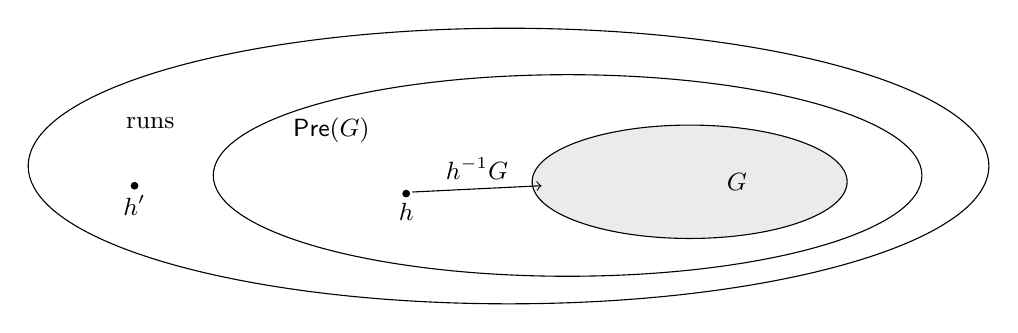
\begin{tikzpicture}[font=\small]
  \draw (0,0) ellipse (6.1 and 1.75);
  \draw (0.75,-0.12) ellipse (4.5 and 1.28);
  \draw[fill=black!8] (2.3,-0.2) ellipse (2.0 and 0.72);
  \node at (-4.55,0.55) {runs};
  \node at (-2.25,0.45) {$\pre{G}$};
  \node at (2.9,-0.2) {$G$};
  \fill (-1.3,-0.35) circle (1.4pt) node[below] {$h$};
  \draw[->] (-1.22,-0.33) -- node[above] {$h^{-1}G$} (0.42,-0.25);
  \fill (-4.75,-0.25) circle (1.4pt) node[below] {$h'$};
\end{tikzpicture}
\caption{The runs that the plan allows and that break no obligation, the beginnings of goal
runs, and the goal. A harness can enforce the middle set, and no smaller one that contains the goal. At a stop
after $h$, the report denotes $h^{-1}G$, the ways to finish. After $h'$ there is none: the shield
refuses the letter that leads there.}
\Description{Three nested ellipses. The outer one is the set of runs, the middle one the set
of beginnings of goal runs, the inner one the goal. A point h lies in the middle set with an
arrow into the goal that is labelled with the quotient. A point h prime lies in the outer set
only.}
\label{fig:sets}
\end{figure}

The work is the counterpart of an earlier paper of this series, which made permissions
languages~\cite{tpp11}. A permission is used up by the actions that it allows, it may be left
unused, and it is closed under beginnings. An obligation is the opposite on each count: an
action that serves one obligation serves every obligation that watches it, an obligation may
not be left, and what satisfies it is closed under continuations. The two meet in the
shield.

None of the proofs is long. Each result rests on a classical notion: the derivative, the
closure of a property, the quotient of a language and the equivalence of
\citet{nerode1958}, the nonblocking supervisor of \citet{ramadge1987}, the frame rule. What
we claim as new is that together they answer the question what a harness can do about work
that an agent may leave, the least request, the frame condition for obligations, and the
evidence from a session that was not staged.

\section{Overview}
\label{sec:overview}

Consider an agent that maintains one paper in a repository like ours. Six actions matter,
and we write them as letters: $\edit$ changes the source, $\tex$ compiles it and yields a
PDF, $\commit$ and $\push$ record and publish the change, $\pull$ fetches what others have
pushed, and $\look$ reads the registry in which a robot assigns numbers to papers. Two
standing instructions apply:
\[
  \edit \;\creates\; \tex \bef \commit
  \qquad\qquad
  \commit \;\creates\; \push \later \pull \later \look
\]
The first says that an edit creates an obligation: a compilation must come before the next
commit. The second says that a commit creates the obligation to push, later to pull, and
later to look; we read $\later$ as ``and later''. The person has approved a plan. The agent
may edit, compile, commit, pull, and look as often as it likes, and it may push once:
\[
  P \;=\; (\edit + \tex + \commit + \pull + \look)^{*} \sh \push .
\]

\begin{table}
\caption{A run of the example. The agent proposes one letter at a time. The fourth column
shows the ledger after the step, and the last column the number of letters that are still
needed at least.}
\label{tab:walk}
\begin{tabular}{rlp{5.6cm}lr}
\toprule
 & letter & shield & open afterwards & left \\
\midrule
\rows{walk}
\bottomrule
\end{tabular}
\end{table}

\paragraph{The ledger.} Table~\ref{tab:walk} shows a run. After step~1 the ledger has one
entry, $\tex \bef \commit$, and step~3 meets it. The commit of step~4 creates the entry
$\push \later \pull \later \look$. An entry is a language, here the words in which the three
letters occur in this order. With the push of step~5 the ledger replaces the language by its
derivative, the words that may follow a push, and the entry reads $\pull \later \look$.
After the pull it reads $\look$, and the look removes it.

\paragraph{Stops.} Suppose that the run stops after step~4. The report is the open part of
the ledger: $\push \later \pull \later \look$, owed since step~4. If it stops after step~6,
the report is $\look$. Whoever continues, be it the same model after its context was
summarized, another agent, or the user, needs to know nothing else about the past to judge
what follows. The harness computes the report from the actions that it saw. What the model says about its own work plays no part.

\paragraph{Refusals.} \claim{walk-refusals}{The shield refuses two letters of the run.} At
step~2 the agent proposes a commit while $\tex \bef \commit$ is open. The commit would break
the obligation for good, and no continuation could repair it. At step~10 the commit breaks
nothing and the plan allows it. But it would create $\push \later \pull \later \look$, and
the one push of the plan was spent at step~5: no run of the plan could discharge the new
obligation. The shield refuses, and it tells the agent the least that it would have to ask
the person for, which is one more push. Without the shield the commit would happen, and the
next report would contain an obligation that nobody who holds this plan can meet.

The shield does not make the agent push after step~4. If the agent stops there, the stop is
allowed and the report says what is left. Because of the shield, what is left can be done
under the plan that is left. The example has \exExampleStates{} states, and
\exExampleCovered{} of them have this property; the shield keeps the run among those.

\section{Obligations and the Ledger}
\label{sec:ledger}

\subsection{Letters and Expressions}

A \emph{letter} is an action as the harness observes it, with as much of its outcome as
matters: $\tex$ stands for a compilation that produced a PDF, and a compilation that failed
is not a letter. Letters are observations of the harness, not statements of the
model~\cite{tpp10}. We fix a finite set $\Sigma$ of letters. Words, ranged over by $h$, $u$,
$v$, $w$, are finite sequences of letters. The projection $\proj{w}{W}$ of a word to a set
$W$ of letters erases the letters outside $W$. For a language $L$, $\pre{L}$ is the set of
the beginnings of its words, and $w^{-1}L = \{v \mid wv \in L\}$ is its quotient by $w$.

Expressions are regular expressions with the shuffle of two languages, which contains every
interleaving of a word of the first with a word of the second:
\[
  r \;::=\; \emptyset \mid \varepsilon \mid a \mid r \cdot r \mid r + r \mid r^{*} \mid r \sh r .
\]
We write $\lang{r}$ for the language of $r$, and a finite set of letters stands for the sum
of its elements. The derivative $\dv{a}{r}$ of an expression by a letter is an expression
for $a^{-1}\lang{r}$, computed from the syntax~\cite{brzozowski1964}; $\dv{u}{r}$ is the
derivative by the letters of $u$ in turn. An expression has finitely many derivatives up to
the laws of the sum; with the shuffle, a derivative of $r \sh r'$ is a sum of shuffles of
derivatives of $r$ and of $r'$. It is decidable from the syntax whether
$\lang{r}$ is empty and whether it contains $\varepsilon$.

\subsection{Obligations}

\begin{definition}[Obligation]
\label{def:ob}
An obligation is a pair $o = \ob{r}{W}$ of a set $W \subseteq \Sigma$ of \emph{watched}
letters and an expression $r$ over $W$ whose language is not empty and does not contain
$\varepsilon$. Let $w$ be a word and $u = \proj{w}{W}$. After $w$, the obligation is
\begin{itemize}
\item \emph{met} if a beginning of $u$ is in $\lang{r}$,
\item \emph{broken} if it is not met and $u$ is not in $\pre{\lang{r}}$,
\item \emph{open} otherwise.
\end{itemize}
It is \emph{settled} at the $n$th letter of $w$ if it is met or broken after the first $n$
letters of $w$ and open after the first $n - 1$.
\end{definition}

An obligation sees only its watched letters. It is met by the first watched word that is in
its language, and it is broken by a watched letter that its language does not expect at that
point. Both verdicts are final: when a beginning of $u$ is in $\lang{r}$ it stays a
beginning of every longer word, and when $u$ is not in $\pre{\lang{r}}$, no longer word is.
Among the properties of infinite runs, those that a finite beginning settles for good in
the positive are the guarantee properties of \citet{manna1990}, and such a beginning is a
good prefix in the sense of \citet{kupferman2001}.

Two shapes cover the rules of this paper. For letters $a$ and $b$,
\[
  a \bef b \;=\; \ob{a}{\{a, b\}}
\]
is met by $a$ and broken by a $b$ that comes first. The watched letters that the expression
never expects act as deadlines. For distinct letters $a_1, \ldots, a_n$ with
$A = \{a_1, \ldots, a_n\}$,
\[
  a_1 \later \cdots \later a_n \;=\;
  \ob{(A \setminus a_1)^{*} \cdot a_1 \cdot (A \setminus a_2)^{*} \cdot a_2 \cdots (A \setminus a_n)^{*} \cdot a_n}{A}
\]
waits for $a_1$, then for $a_2$, and so on, and ignores the other letters of $A$ while it
waits. No letter breaks it. The single letter $a$ abbreviates $\ob{a}{\{a\}}$.

The ledger does not test membership of growing words. It moves an obligation by one letter:
\[
  \ob{r}{W} \cdot a \;=\;
  \begin{cases}
    \ob{r}{W} & \text{if } a \notin W \\
    \met & \text{if } a \in W \text{ and } \varepsilon \in \lang{\dv{a}{r}} \\
    \brk & \text{if } a \in W \text{ and } \lang{\dv{a}{r}} = \emptyset \\
    \ob{\dv{a}{r}}{W} & \text{otherwise}
  \end{cases}
\]
and $\met \cdot a = \met$, $\brk \cdot a = \brk$. We write $o \cdot w$ for the result of
moving $o$ by the letters of $w$ in turn.

\begin{lemma}
\label{lem:step}
Let $o = \ob{r}{W}$ be an obligation, $w$ a word, and $u = \proj{w}{W}$. If $o$ is open after
$w$ then $o \cdot w = \ob{\dv{u}{r}}{W}$. It is met after $w$ exactly if $o \cdot w = \met$
and broken exactly if $o \cdot w = \brk$, and the letter at which the moves first yield the
verdict is the letter at which $o$ is settled.
\end{lemma}

\begin{proof}
By induction on $w$. After the empty word $o$ is open, because $\varepsilon \notin
\lang{r}$ and $\lang{r}$ is not empty, and $o \cdot \varepsilon = o$. Let $o$ be open after
$w$, so that no beginning of $u$ is in $\lang{r}$ and $o \cdot w = \ob{\dv{u}{r}}{W}$, and
let $a$ be a letter. If $a \notin W$ then the projection, the status, and the obligation
stay the same. If $a \in W$ then $o$ is met after $wa$ exactly if $ua \in \lang{r}$, which
is $\varepsilon \in \lang{\dv{ua}{r}}$. It is broken exactly if it is not met and
$ua \notin \pre{\lang{r}}$, which is $\lang{\dv{ua}{r}} = \emptyset$. Otherwise it is open
and $o \cdot wa = \ob{\dv{ua}{r}}{W}$. If $o$ is settled after $w$, both sides keep the
verdict.
\end{proof}

\subsection{Rules and the Ledger}

Obligations come from two sources. Some are in the ledger when the work starts: the request
of the user, or the report of a predecessor. The others are created by \emph{rules}. A set
of rules is a function $\rules$ that maps every letter $a$ to a finite list $\rules(a)$ of
obligations, those that performing $a$ creates. We write $a \creates o$ for
$o \in \rules(a)$. A rule is the form of a standing instruction of the kind ``after every
$a$, do $o$'', the response pattern of \citet{dwyer1999}. A rule with a parameter, such as
$\edit_p \creates \tex_p \bef \commit_p$ for every paper $p$, stands for one rule for each
value of the parameter.

\begin{definition}[Entries]
\label{def:entries}
Let $\Omega_0$ be a list of obligations and $h = a_1 \cdots a_n$ a history. The
\emph{entries} of $h$ are the pairs $(0, o)$ for $o$ in $\Omega_0$ and $(i, o)$ for
$1 \le i \le n$ and $o$ in $\rules(a_i)$. The entry $(i, o)$ is met, broken, or open after
$h$ according as $o$ is after $a_{i+1} \cdots a_n$.
\end{definition}

An obligation watches what happens after its creation. In particular, the letter that
creates it does not count for it. The \emph{ledger} is the machine that one expects. It
holds the open entries, each with an obligation that changes over time, and a record of the
closed ones. To read a letter $a_i$ it moves the obligation of every open entry by $a_i$,
transfers the entries whose obligation became $\met$ or $\brk$ to the record together with
the verdict and the index $i$, and then adds the entries $(i, o)$ for $o$ in $\rules(a_i)$.

\begin{theorem}[The ledger is right]
\label{thm:ledger}
Let $\Omega_0$ be a list of obligations and $h = a_1 \cdots a_n$ a history. After reading
$h$, the open entries of the ledger are the entries of $h$ that are open after $h$. The
ledger holds the entry $(i, \ob{r}{W})$ with the obligation $\ob{\dv{u}{r}}{W}$, where $u$
is the projection of $a_{i+1} \cdots a_n$ to $W$. The record holds the entries that are met
and those that are broken, each with the index of the letter at which it was settled.
\end{theorem}

\begin{proof}
The ledger moves the obligation of the entry $(i, o)$ by the letters $a_{i+1}, \ldots, a_n$
and by no other, because it adds the entry after it has read $a_i$. The claim is
Lemma~\ref{lem:step} for $o$ and the word $a_{i+1} \cdots a_n$.
\end{proof}

\subsection{Reports and Stops}

\begin{definition}[Report]
The \emph{report} after a history $h$ lists the open entries of the ledger, each with its
index, the letter that created it, and the obligation that the ledger holds for it. We call
that obligation what is \emph{left} of the entry.
\end{definition}

\begin{proposition}[A report is enough]
\label{prop:enough}
Let $h$ be a history with $n$ letters and $v$ a word. Start a second ledger with the
obligations that are left of the open entries after $h$, and let it read $v$. Then every
entry that is open after $h$ has the same verdict after $hv$ in the first ledger as its
counterpart has after $v$ in the second, settled at letters whose indices differ by $n$. The
entries that $v$ creates are the same in both.
\end{proposition}

\begin{proof}
Let $(i, \ob{r}{W})$ be open after $h$, and let $u$ be the watched part of what follows
$a_i$ in $h$. By Theorem~\ref{thm:ledger} what is left of it is $\ob{\dv{u}{r}}{W}$, and no
beginning of $u$ is in $\lang{r}$. So a beginning of $u \cdot \proj{v}{W}$ is in $\lang{r}$
exactly if a beginning of $\proj{v}{W}$ is in $u^{-1}\lang{r} = \lang{\dv{u}{r}}$, and
$u \cdot \proj{v}{W}$ is in $\pre{\lang{r}}$ exactly if $\proj{v}{W}$ is in
$\pre{\lang{\dv{u}{r}}}$. The entries that $v$ creates depend on $v$ alone.
\end{proof}

A run may stop after any of its letters. Theorem~\ref{thm:ledger} holds for every history,
so it holds at every stop, and no assumption is needed about how a run ends.

\begin{corollary}[Every stop has a right report]
\label{cor:stop}
At every stop, every obligation that was in the ledger at the start or was created since is
met, broken, or open, and exactly one of the three. The record says which obligations are
met and which are broken, and when. The report lists the open ones with what is left of
each, and by Proposition~\ref{prop:enough} that is all that their future depends on.
\end{corollary}

That the report is right is a property of every beginning of every run, and the harness
establishes it alone. That the report is empty is not such a property, and the next section
turns to it.

The four kinds of stop differ only in who receives the report. When a turn ends, the harness
shows it to the user next to the last message of the model. When the context is summarized,
the harness puts it into the new context after the summary; the ledger is kept outside the
context and is not summarized. When work is handed to another agent, the obligations that
go with it are entries of that agent's ledger, and its report returns with its result
(Section~\ref{sec:frame}). When the process dies, nothing is lost that a journal does not
restore: the ledger is a function of the letters, so a harness that keeps a durable journal
of the actions that it performed~\cite{tpp8} rebuilds it.

\section{Goals, Coverage, and the Shield}
\label{sec:shield}

\subsection{States and Goals}

The agent acts under a \emph{plan}, an expression $P$. The plan allows a history $h$ when
$h$ is the beginning of a word of $P$. After a letter $a$ the agent holds $\dv{a}{P}$, what
is left of the plan~\cite{tpp11}. Plans may use the shuffle: the plan $P \sh a$ allows what
$P$ allows and the letter $a$ once, at any time. A \emph{state} $s = \st{P}{\Omega}$ is a
plan and the set $\Omega$ of the obligations that are left of the open entries. The names of
the entries play no role for what can happen next, and two entries with the same obligation
count once. A state steps by a letter when the plan allows the letter and no obligation
breaks:
\[
\inferrule*[right=Step]
  {\lang{\dv{a}{P}} \neq \emptyset \\ o \cdot a \neq \brk \text{ for all } o \in \Omega}
  {\st{P}{\Omega} \step{a} \st{\dv{a}{P}}{(\{o \cdot a \mid o \in \Omega\} \setminus \{\met\}) \cup \rules(a)}}
\]
We write $s \step{w} s'$ for a sequence of steps, and $s \cdot w$ for $s'$, which is unique
when it exists. From a state only finitely many states can be reached, because an expression
has finitely many derivatives.

\begin{definition}[Goal]
\label{def:goal}
The goal of a state $s$ is the set of words that lead from it to an empty ledger:
\[
  \goal{s} \;=\; \{ w \mid s \step{w} \st{P'}{\emptyset} \text{ for some } P' \} .
\]
\end{definition}

By Theorem~\ref{thm:ledger}, a word $w = a_1 \cdots a_n$ is in $\goal{\st{P}{\Omega}}$
exactly if it is in $\pre{\lang{P}}$, every obligation of $\Omega$ is met after $w$, and for
every $i$ every obligation of $\rules(a_i)$ is met after $a_{i+1} \cdots a_n$. The goal need
not be closed under continuations: a goal word followed by a letter that creates an
obligation is no goal word.

\begin{proposition}[The state is the quotient]
\label{prop:quotient}
Let $s$ be a state and $h$ a history.
\begin{enumerate}
\item If $s \step{h} s'$ then $\goal{s'} = h^{-1}\goal{s}$. If $h$ has no steps from $s$ then
  $h^{-1}\goal{s}$ is empty.
\item Two histories $h_1$ and $h_2$ satisfy $h_1 v \in \goal{s} \Leftrightarrow h_2 v \in
  \goal{s}$ for every word $v$ exactly if $\goal{s \cdot h_1} = \goal{s \cdot h_2}$, where
  the goal of a state that does not exist is empty. It is decidable whether they do.
\item Let $f$ be a function on histories with $f(h_1) = f(h_2)$ for two histories that
  differ in the sense of (2). Then there is a word $v$ such that exactly one of $h_1 v$ and
  $h_2 v$ is in $\goal{s}$.
\end{enumerate}
\end{proposition}

\begin{proof}
(1) Steps are deterministic, so $s \step{hv} \st{P'}{\emptyset}$ exactly if
$s' \step{v} \st{P'}{\emptyset}$. (2) By (1) both sides say $h_1^{-1}\goal{s} =
h_2^{-1}\goal{s}$. The states that are reachable from $s$, with the test for an empty
ledger, form a finite deterministic automaton for $\goal{s}$, and the equivalence of two of
its states is decidable. (3) is the definition of (2).
\end{proof}

Part (2) is the equivalence of \citet{nerode1958} for the language $\goal{s}$. Part (3) says
that a successor that is told less than the class of the history, by a summary $f$, can be
wrong about whether a continuation finishes the work. The state that the history leads to,
which is the plan that is left and the report without its names, determines the class.
\claim{different-ledgers}{The converse fails: states with different ledgers can have one
goal.} The simplest case is a ledger with one more obligation that is met whenever another
one is.

\subsection{Coverage and the Shield}

\begin{definition}[Covered]
A state $s$ is \emph{covered} if $\goal{s}$ is not empty.
\end{definition}

In a covered state some word that the plan allows meets every open obligation and every
obligation that the word itself creates. This is the principle that what is owed is allowed,
for all obligations at once and with the consequences of meeting them.

\begin{lemma}
\label{lem:mono}
If $\st{P}{\Omega}$ is covered, $\Omega' \subseteq \Omega$, and $\pre{\lang{P}} \subseteq
\pre{\lang{P'}}$, then $\st{P'}{\Omega'}$ is covered.
\end{lemma}

\begin{proof}
A word of $\goal{\st{P}{\Omega}}$ is allowed by $P'$. The obligations move independently of
each other, so those of $\Omega'$ are met as before, and the word creates the same
obligations as before.
\end{proof}

So coverage survives when the user waives an obligation and when the user grants a further
plan $Q$, which turns $P$ into $P \sh Q$.

\begin{definition}[Shield]
In a covered state $s$, the \emph{shield} allows the letter $a$ if $s \step{a} s'$ and $s'$
is covered. It never refuses a stop. A request to add an obligation $o$ to the ledger of
$\st{P}{\Omega}$ is accepted if $\st{P}{\Omega \cup \{o\}}$ is covered.
\end{definition}

A \emph{mechanism} is a set $M$ of histories that is closed under beginnings: the histories
that some harness lets happen from a given state when it decides about each letter and
cannot prevent a stop. These are the sets that refusals can enforce~\cite{schneider2000}.

\begin{theorem}[The shield]
\label{thm:shield}
Let $s$ be a covered state.
\begin{enumerate}
\item The histories that the shield allows from $s$ are the words of $\pre{\goal{s}}$.
\item Let $M$ be a mechanism. If $M$ contains every word of $\goal{s}$, then $M$ contains
  every history that the shield allows. If every history of $M$ leads from $s$ to a covered
  state, then the shield allows every history of $M$. So the shield is the only mechanism
  with both properties.
\item In every state that the shield reaches, the ledger is empty or the shield allows a
  letter. A shortest word of the goal of a state has fewer letters than there are states
  reachable from it.
\item If a shielded run stops after $h$ in the state $s'$, then $s'$ is covered and
  $\goal{s'} = h^{-1}\goal{s}$.
\end{enumerate}
\end{theorem}

\begin{proof}
We first show that $s \cdot h$ exists and is covered exactly if $h \in \pre{\goal{s}}$. If
$s \cdot h$ is covered, some $v$ is in $\goal{s \cdot h} = h^{-1}\goal{s}$, so $hv \in
\goal{s}$. If $hv \in \goal{s}$ then the steps of $h$ exist and $v \in \goal{s \cdot h}$.
(1) The shield allows $h$ exactly if for every beginning $h'$ of $h$ the state $s \cdot h'$
exists and is covered, which is $h' \in \pre{\goal{s}}$ for all of them, which is
$h \in \pre{\goal{s}}$. (2) A set that is closed under beginnings and contains $\goal{s}$
contains $\pre{\goal{s}}$. If every history of $M$ leads to a covered state, then
$M \subseteq \pre{\goal{s}}$ by the first sentence of the proof. (3) Let the ledger of a
covered state $t$ be nonempty. Then the empty word is not in $\goal{t}$, a word $av$ is, and
$v \in \goal{t \cdot a}$, so the shield allows $a$. A shortest word of the goal visits no
state twice. (4) is (1) and Proposition~\ref{prop:quotient}.
\end{proof}

Part (2) is the sense in which the shield is all that refusals can do for the goal. The
first property says that the mechanism loses no successful run. The second says that it
leaves no report that cannot be finished. A mechanism that allows more than the shield
allows a history after which the goal is out of reach. A mechanism that allows less refuses
the beginning of a run that would have reached the goal. In terms of
\citet{alpern1985}, $\pre{\goal{s}}$ is the smallest safety property that every goal run
satisfies, and by part (4) the gap between it and the goal is filled at every stop by a
report that denotes the ways to finish.

\begin{corollary}[What is owed is allowed]
\label{cor:owed}
In a shielded run that starts in a covered state, no obligation is ever broken, and at
every moment some word that the plan allows meets every open obligation and every obligation
that it creates. Whoever receives the report of a stop together with the plan that is left
can empty the ledger.
\end{corollary}

In the run of Table~\ref{tab:walk} the shield refuses the commit of step~2 because the step
does not exist, and the commit of step~10 because the state that the step leads to is not
covered. It allows the commit of step~4 because the plan still has the push that the new
obligation needs.

\subsection{The Least Request}

When a state is not covered, the agent can ask the person for more authority, and the
harness can say for what. A \emph{request} is a finite multiset $E = \{e_1, \ldots, e_k\}$ of
letters. Granting it to $\st{P}{\Omega}$ gives $\st{P \sh e_1 \sh \cdots \sh e_k}{\Omega}$:
each letter of the request may be performed once, at any time. A \emph{least request} of a
state is a request of the least size whose grant makes the state covered.

\begin{theorem}[Least request]
\label{thm:ask}
Consider the graph whose nodes are the states and that has, for every letter $a$, an edge
of cost 0 from $t$ to $t \cdot a$ when the step exists, and an edge of cost 1 from
$\st{Q}{\Omega_1}$ to $\st{Q}{\Omega_2}$ when $\st{\Sigma^{*}}{\Omega_1} \step{a}
\st{\Sigma^{*}}{\Omega_2}$. The least cost of a path from $s = \st{P}{\Omega}$ to a state
with an empty ledger is the size of a least request of $s$, and the letters of the edges of
cost 1 on such a path form one. There is no such path exactly if
$\st{\Sigma^{*}}{\Omega}$ is not covered, and then no request makes $s$ covered.
\end{theorem}

\begin{proof}
An edge of cost 1 performs a letter that the request pays for: the ledger moves and the plan
stays. A word is in $\pre{\lang{P \sh e_1 \sh \cdots \sh e_k}}$ exactly if it is an
interleaving of a word of $\pre{\lang{P}}$ with some of the letters $e_1, \ldots, e_k$. So
the paths to an empty ledger whose edges of cost 1 carry letters among $e_1, \ldots, e_k$,
each at most as often as it occurs in $E$, are the words of the goal of the granted state.
If $\st{\Sigma^{*}}{\Omega}$ is covered by a word, the request that consists of its letters
covers $s$, and if a request covers $s$ then the same word covers
$\st{\Sigma^{*}}{\Omega}$.
\end{proof}

A letter that the plan allows may have to be asked for nonetheless.
\claim{ask-example}{Under the plan $a + b \cdot b$ with the open obligation
$\ob{a \cdot b \cdot b}{\{a, b\}}$, performing $a$ by the plan leaves nothing for the two
letters $b$, and they would have to be asked for. The least request is one $a$, after which
the plan pays for both $b$.}

A stop in a run without a shield is thus of one of three kinds. If the state is covered, the
work can be finished with what the agent holds. If it has a nonempty least request, the work
is blocked, and the request says by what. If no request helps, or the record contains a
broken obligation, something is lost: the open obligations exclude each other, or a
deadline has passed.

\subsection{Cost}

\begin{proposition}
\label{prop:cost}
It is decidable whether a state is covered. The problem is hard for polynomial space when
the languages of the obligations are given by deterministic automata, even with no rules and the plan
$\Sigma^{*}$. With the plan given by a nondeterministic automaton as well, it is in
polynomial space.
\end{proposition}

\begin{proof}
The states that are reachable from a state are finitely many, which decides coverage. For
the lower bound we reduce from the question whether deterministic automata $A_1, \ldots,
A_k$ over an alphabet $\Gamma$ accept a common word, which is complete for polynomial
space~\cite{kozen1977}. We may assume that each of them accepts some word. Let \$ be a new
letter, and let $o_i$ be the obligation that watches $\Gamma \cup \{\$\}$ and whose language
is $\lang{A_i} \cdot \$$. After a word $x \$ y$ with $x \in \Gamma^{*}$, the obligation
$o_i$ is met if $x \in \lang{A_i}$ and broken otherwise, and after a word without \$ it is
not met. So $\st{\Sigma^{*}}{\{o_1, \ldots, o_k\}}$ is covered exactly if some $x$ is in
every $\lang{A_i}$. For the upper bound, an open obligation is a state of one of the given
automata, so a ledger is a set of such states, and a state of the system is a ledger
together with a state of the automaton of the plan. A search that guesses a word letter by
letter keeps one state of the system and a counter.
\end{proof}

\begin{table}
\caption{Obligations that are cheap to state and expensive to meet together. The $i$th
obligation is met by a positive multiple of the $i$th prime number of letters $a$ followed by
the letter $z$.}
\label{tab:primes}
\begin{tabular}{rrrr}
\toprule
obligations & letters in their expressions & shortest word of the goal & reachable states \\
\midrule
\rows{primes}
\bottomrule
\end{tabular}
\end{table}

Table~\ref{tab:primes} shows the growth on a small family. \claim{primes-product}{The
shortest word that meets the first $k$ obligations has one letter more than the product of
the first $k$ primes}, while the expressions grow with their sum: four obligations of
\exPrimesLetters{} letters need \exPrimesLength{}. The number of open obligations that
interact is what makes coverage expensive. The next section shows when they do not interact.

\section{Two Agents and the Frame Condition}
\label{sec:frame}

An agent hands work to another agent, or two sessions work in one repository. Each has a
plan and a ledger, and they act in one world: an open obligation sees every letter that it
watches, whoever performs it. A joint state is a pair of states $s_1 = \st{P_1}{\Omega_1}$
and $s_2 = \st{P_2}{\Omega_2}$. Agent $i$ steps by a letter $a$ when $\dv{a}{P_i}$ is not
empty and no obligation of either ledger breaks. Then $P_i$ becomes $\dv{a}{P_i}$, both
ledgers move by $a$, and the obligations $\rules(a)$ join the ledger of agent $i$, who
caused them. The joint state is covered if some sequence of steps of the two agents empties
both ledgers, and the joint shield allows a step if it leads to a covered joint state.

Deciding about one agent by looking at both is expensive, and it is wrong in spirit: an
agent to which a part was handed should not need to know the rest. The condition under
which it need not is that the agents keep out of each other's sight. Let $\letters{P}$ be
the letters that occur in $P$.

\begin{definition}[Separated]
\label{def:sep}
For a state $s = \st{P}{\Omega}$, let $\watch{s}$ be the union of the watched sets of the
obligations of $\Omega$ and of the obligations of $\rules(a)$ for all $a \in \letters{P}$.
Two states $s_1$ and $s_2$ are \emph{separated} if $\letters{P_1} \cap \watch{s_2}$ and
$\letters{P_2} \cap \watch{s_1}$ are empty.
\end{definition}

\begin{theorem}[Frame]
\label{thm:frame}
Let $s_1$ and $s_2$ be separated.
\begin{enumerate}
\item A step of either agent leads to a joint state that is separated, and it leaves the
  state of the other agent as it was.
\item The joint state is covered exactly if $s_1$ is covered and $s_2$ is covered.
\item In a covered joint state, the joint shield allows agent $i$ the letter $a$ exactly if
  the shield of $s_i$ alone allows $a$.
\end{enumerate}
\end{theorem}

\begin{proof}
(1) Let agent 1 step by $a$. Then $a \in \letters{P_1}$, so no obligation of $\Omega_2$
watches $a$, and $\Omega_2$ and $P_2$ stay. The new ledger of agent 1 consists of
obligations that were moved, which keep their watched sets, and of obligations of
$\rules(a)$, whose watched sets are in $\watch{s_1}$ by definition. The letters of
$\dv{a}{P_1}$ are among those of $P_1$. So $\watch{s_1}$ and $\letters{P_1}$ do not grow.
(2) Let steps of the two agents empty both ledgers, and let $w_i$ be the letters of agent
$i$ in them, in order. An obligation of agent 1, from $\Omega_1$ or created by a letter of
$w_1$, watches no letter of $w_2$, so it sees in the joint run what it sees in $w_1$ alone,
and $w_1 \in \goal{s_1}$. Conversely, let $w_i \in \goal{s_i}$. Let agent 1 perform $w_1$
and then agent 2 perform $w_2$. During $w_1$ the ledger of agent 2 stays as it is, and the
ledger of agent 1 becomes empty as it does alone. During $w_2$ no obligation of agent 1 is
left to be broken. (3) By (1) the step of agent $i$ exists jointly exactly if it exists
alone, and it leads to a separated joint state whose other half is unchanged and, by (2),
covered. By (2) again the new joint state is covered exactly if the new state of agent $i$
is.
\end{proof}

The theorem has the shape of the frame rule of separation logic~\cite{reynolds2002,
ohearn2007}: what an agent does not touch stays true, and so it need not be looked at. It
gives the rule for handing over. An obligation moves to another agent only together with a
plan that covers it, and the two parts must be separated afterwards. The sub-agent is then
shielded by its own ledger. When it stops, its report and what is left of its plan come back
covered by Theorem~\ref{thm:shield}, and the pair is covered by part (2).
\claim{not-separated-differ}{Without separation part (2) fails in both directions.} Two
agents can each be covered alone and not together, when every way for one of them to finish
breaks an obligation of the other. And they can be covered together and not alone, when one
performs what the other owes.

Separation also saves work. \claim{copies-multiply}{Two copies of the example of
Section~\ref{sec:overview} with letters of their own have \exCopiesTwo{} joint states and
three copies have \exCopiesThree{}}, the powers of the \exExampleStates{} states of one
copy. The copies are separated, so three shields that look at \exApartThree{} states in all
decide the same.

\section{Code That Is Checked Before It Runs}
\label{sec:code}

The shield asks whether some word finishes the work. That is the right question for an
agent that chooses its next letter, because the agent can choose that word. It is the wrong
question for a piece of code that the model writes and that then runs on its own: a script,
a loop over files, a hook. At a branch of such code the world decides, by the result of a
test or the failure of a command. An earlier paper of this series checks the type of such
code against the approvals that it is given, before it runs~\cite{tpp4}. Here the check
concerns what the code leaves open.

\emph{Code} is an expression without shuffle and without $\emptyset$, read as a program: $c \cdot d$ runs $c$ and
then $d$, $c + d$ runs one of the two, and $c^{*}$ runs $c$ some number of times. The words
of $\lang{c}$ are the runs of $c$. Figure~\ref{fig:code} defines a judgment
$S \vdash c \dashv S'$ between finite sets of states: started in a state of $S$, every run of
$c$ is allowed and ends in a state of $S'$.

\begin{figure}
\begin{mathpar}
\inferrule*[right=Skip]{ }{S \vdash \varepsilon \dashv S}
\and
\inferrule*[right=Act]
  {s \step{a} s \cdot a \text{ for all } s \in S}
  {S \vdash a \dashv \{s \cdot a \mid s \in S\}}
\and
\inferrule*[right=Seq]
  {S \vdash c \dashv S' \\ S' \vdash d \dashv S''}
  {S \vdash c \cdot d \dashv S''}
\and
\inferrule*[right=Choice]
  {S \vdash c \dashv S_1 \\ S \vdash d \dashv S_2}
  {S \vdash c + d \dashv S_1 \cup S_2}
\and
\inferrule*[right=Loop]
  {S \subseteq I \\ I \vdash c \dashv I' \\ I' \subseteq I}
  {S \vdash c^{*} \dashv I}
\end{mathpar}
\caption{The check of code. $S$, $S'$, and $I$ are finite sets of states.}
\Description{Five inference rules: Skip, Act, Seq, Choice and Loop. Act requires that every
state of the set has a step by the letter. Loop requires a set of states that contains the
start and that the body maps into itself.}
\label{fig:code}
\end{figure}

\begin{theorem}[The check is sound and complete]
\label{thm:code}
Let $S$ be a finite set of states and $c$ code. Write $\post{S}{c}$ for the set of the
states $s \cdot w$ with $s \in S$ and $w \in \lang{c}$.
\begin{enumerate}
\item If $S \vdash c \dashv S'$ then for all $s \in S$ and $w \in \lang{c}$ the state
  $s \cdot w$ exists and is in $S'$.
\item If $s \cdot w$ exists for all $s \in S$ and $w \in \lang{c}$, then $\post{S}{c}$ is
  finite and $S \vdash c \dashv \post{S}{c}$.
\end{enumerate}
It is decidable whether the condition of (2) holds, and when it fails, the beginning of a
run of $c$ and the letter at which the run is refused can be computed.
\end{theorem}

\begin{proof}
Both parts are by induction on $c$. The interesting case is the loop. (1) By induction on
the number of rounds, every run of $c^{*}$ from a state of $S \subseteq I$ ends in $I$:
after no round it ends where it starts, and a further round leads from $I$ to $I' \subseteq
I$. (2) Let $I = \post{S}{c^{*}}$, which is finite because the reachable states are. A state
of $I$ is $s \cdot u$ for a run $u$ of $c^{*}$, and for a run $w$ of $c$ the word $uw$ is a
run of $c^{*}$, so $s \cdot uw$ exists. By the induction hypothesis $I \vdash c \dashv
\post{I}{c}$, and $\post{I}{c} \subseteq I$. For the decision, compute $\post{S}{c}$ along
the syntax, with the least set that contains the start and is closed under the body for a
loop, and stop at the first letter for which some state has no step.
\end{proof}

\begin{theorem}[Checked code is not stopped]
\label{thm:erase}
Let $\{s\} \vdash c \dashv S'$ and let every state of $S'$ be covered. Then for every run $w$
of $c$ and every beginning $u$ of $w$, the state $s \cdot u$ is covered. So the shield
allows every letter of every run of $c$, and wherever a run of $c$ is cut short, the report
can be finished.
\end{theorem}

\begin{proof}
Let $w = uv$. By Theorem~\ref{thm:code} the state $s \cdot w$ exists and is in $S'$, so some
word $x$ is in its goal, and $vx$ is in the goal of $s \cdot u$.
\end{proof}

The code needs no shield while it runs, which matters when a refusal in the middle of a
script would leave more undone than the script was meant to do. And the set $S'$ is a
summary of the code that a harness can show before the run: the reports with which the code
can end.

\begin{table}
\caption{The exits of the script that shipped the papers of the session, started with an
edited paper and a changed artifact. Each line is one way in which the script ends, with
the letters that it has performed and the ledger that it leaves.}
\label{tab:exits}
\begin{tabular}{ll}
\toprule
performed & open at the exit \\
\midrule
\rows{exits}
\bottomrule
\end{tabular}
\end{table}

\paragraph{The script that shipped our papers.} In the session of
Section~\ref{sec:session}, a short script shipped each paper. It compiles the paper,
runs the artifact, commits, pulls with a rebase, and pushes, and it exits at the first
command that fails. As code, with the letters $\code$ and $\run$ for changing and running an
artifact and the rule $\code \creates \run \bef \commit$ next to the two rules of
Section~\ref{sec:overview}:
\[
  \varepsilon + \tex \cdot (\varepsilon + \run \cdot (\varepsilon + \commit \cdot (\varepsilon + \pull \cdot \push))) .
\]
A command that fails performs no letter. The check passes, and Table~\ref{tab:exits} lists
the set $S'$: the script has \exShipExits{} exits. The first three leave the ledger no worse
than they found it. The last is the intended one. It leaves $\pull \later \look$ open, which
the script cannot meet, because the robot needs a minute to assign the number.
\claim{ship-one-exit}{One exit, the fourth, leaves a commit without its push}: the script
has committed, the pull has failed, and the script is gone. The pull fails when other files
of the repository have changes that are not committed. \claim{session-tenth}{The session
took this exit once, when the tenth paper was shipped; the next command of the agent stashed
the other changes, pulled, pushed, and restored them.} With a pull that sets such changes
aside by itself, the failure and the exit disappear: \claim{ship-corrected}{the corrected
script has \exShipExitsFixed{} exits and none leaves a push open}.
\claim{bad-script-refused}{A script that commits before it runs the artifact does not pass
the check, which names the commit as the letter that is refused.}

\section{Evaluation}
\label{sec:eval}

The artifact is one Python script of about \exLines{} lines with no dependencies. It implements
expressions with derivatives, obligations, the ledger, states, coverage by a search of the
reachable states, the shield, the least request, the joint system of two agents, and the
check of code. It also implements the definitions a second time in a way that shares only the syntax of
expressions with this: membership in a language is decided by cutting a word in every possible way, without
derivatives, and the verdict of an obligation and the membership of a word in a goal are
read off Definitions~\ref{def:ob} and~\ref{def:goal} with this test. The command
\texttt{make -C artifact check} runs the script and compares its output with the files from
which this paper takes its numbers and the rows of its tables.

\paragraph{Random systems.} A trial draws a system over four letters from a generator with
seed \exSeed{}: rules for some of the letters, obligations with expressions of depth at
most two that watch one to three letters, and a plan that is the shuffle of a part that may
be used without limit and a part that is used up. There are seven kinds of trial, one for
each group of claims, with between \exTrialsShield{} and \exTrialsLedger{} trials each and
\exTrials{} in all.

\emph{The ledger} (\exTrialsLedger{} trials). The ledger reads a random history. Its
\exObligations{} entries, of which \exMet{} end met, \exBroken{} broken, and \exOpen{} open,
are compared with the definition. \claim{ledger-agrees}{Every verdict and the letter at
which it falls agree (Theorem~\ref{thm:ledger}).} At a random point of each history a second
ledger starts from the report, \exHanded{} open obligations in all, and reaches the
verdicts of the first (Proposition~\ref{prop:enough}).

\emph{Coverage} (\exTrialsCover{} trials). For a random state the search decides coverage;
\exCovered{} of the \exStates{} states are covered. A shortest word that the search returns
is checked against the definition of the goal. \claim{cover-agrees}{For the \exSmall{}
states from which at most six states are reachable, a search over all words with at most as many
letters as there are such states, by the definition alone, agrees on whether the goal is empty and on the length of
its shortest word}; this search is complete by Theorem~\ref{thm:shield}(3). The largest
system has \exLargest{} reachable states, and the longest shortest word has \exLongest{}
letters. The same trials test Lemma~\ref{lem:mono}.

\emph{The shield} (\exTrialsShield{} trials). A run under the shield proposes random letters
from a covered start. Of the \exOffered{} letters that were offered, \exAllowed{} were
allowed, \exRefusedPlan{} were refused because the plan forbids them or an obligation would
break, and \exRefusedCover{} because the next state is not covered.
\claim{shield-holds}{Every state of every run is covered, nothing breaks, every run is the
beginning of a goal word by the definition, some letter is allowed whenever the ledger is
not empty, and no refused letter leads to a covered state (Theorem~\ref{thm:shield}).} Of
the \exRuns{} runs, \exStopsReport{} stop with a nonempty report, and a successor finishes
each from the report.

\emph{Requests} (\exTrialsAsk{} trials). \claim{ask-least}{For the \exRequests{} states that
have a least request, the request covers the state and no request with one letter less
does, by a search over all of them (Theorem~\ref{thm:ask}).} \exRequestsNone{} of these
states are covered already, and \exRequestsSome{} need one letter or more. For the other
\exNoRequest{} states no request helps, and the plan $\Sigma^{*}$ does not cover them.

\emph{Two agents} (\exTrialsFrame{} trials). \claim{frame-holds}{For the \exSeparated{}
pairs that are separated, joint coverage and the joint shield agree with the two agents
alone (Theorem~\ref{thm:frame}).} Of the \exNotSeparated{} pairs that are not, \exDiffer{}
disagree.

\emph{Code} (\exTrialsCode{} trials). The check refuses \exPiecesRefused{} pieces of code
and passes \exPiecesPassed{}. \claim{code-holds}{For a refused piece, the run that the check
returns is a run of the piece and is refused at the letter named. For a piece that passes,
every run of at most five letters is allowed and ends in a state that the check reports,
and every reported state is the end of a run (Theorem~\ref{thm:code}).} \exPiecesSafe{}
pieces end only in covered states, and on all their runs of at most five letters every state
on the way is covered (Theorem~\ref{thm:erase}); \exPiecesClosed{} end only with an empty ledger.

\emph{Goals} (\exTrialsEqual{} trials). For two states that histories lead to from one
start, the decision procedure of Proposition~\ref{prop:quotient} either returns a word that
is in one goal and, by the definition, not in the other (\exToldApart{} pairs), or finds the
goals equal (\exSameGoal{} pairs), in which case random words agree. In \exSameGoalOther{} of
the latter pairs the two states differ.

\begin{table}
\caption{Deliberate mistakes and the number of trials after which a test fails.}
\label{tab:mutants}
\begin{tabular}{llr}
\toprule
mistake & test & trials \\
\midrule
an obligation counts letters that it does not watch & ledger & \exTryNoWatch \\
an obligation sees the letter that created it & ledger & \exTrySelfTrigger \\
a watched letter that is not expected is ignored & ledger & \exTryNeverBreak \\
an obligation that is met stays open & ledger & \exTryNoRetire \\
the report lists obligations as they were created & ledger & \exTryStaleReport \\
the shield allows what the plan allows and breaks nothing & shield & \exTryPlanBlind \\
coverage is decided for each obligation alone & shield & \exTrySeparate \\
coverage ignores the obligations that finishing creates & shield & \exTryNoTriggerCover \\
a state counts as finished only when the plan is used up & shield & \exTryNeedComplete \\
a request buys a letter only when the plan forbids it & requests & \exTryGreedyAsk \\
separation ignores the obligations that a plan can create & two agents & \exTryHalfFrame \\
the check runs the body of a loop once & code & \exTryStarOnce \\
the check follows the first branch only & code & \exTryAltFirst \\
\bottomrule
\end{tabular}
\end{table}

\paragraph{Deliberate mistakes.} A test that cannot fail shows nothing. The script has
\exMutants{} switches, each of which plants one mistake in the implementation, and runs the
test for the affected claim until it fails. \claim{all-noticed}{Every mistake is noticed}
(Table~\ref{tab:mutants}). The slowest to show is the request that buys greedily, which
needs \exSlowest{} trials: it takes a plan in which a letter is better kept for later.

\paragraph{What the tests do not show.} The systems are small, with four letters, and the
second implementation of the definitions bounds the length of the words that it tries. The
trials find no counterexample; the theorems are claims about all systems, and their proofs
are in Sections~\ref{sec:ledger} to~\ref{sec:code}.

\section{A Session, Replayed}
\label{sec:session}

The eleven papers before this one were written in one session of an agent in a commercial
harness, over about eight hours. We replayed the session through the ledger.

\paragraph{The trace.} A script reads the record that the harness keeps of the session and
turns the tool calls of the main agent into letters, for every paper $p$: $\edit_p$ when a
source of the PDF is written, $\code_p$ when a source of the artifact is written, $\tex_p$
for a compilation that yields a PDF, $\run_p$ when the artifact is run, $\commit_p$ for a
commit that contains files of the paper, and $\push$, $\pull$, $\look$, and the stashing
and restoring of changes without a paper. A shell command is cut into its parts, and
patterns decide what each part did; we wrote the patterns against the commands of this
session and read the events next to the commands. The record is private. The trace, which
contains nothing but these letters, the names of our papers, and marks for the ends of
turns and for the summaries, is in the artifact. It ends with the third
summary, after the eleventh paper, and has \exSessionLetters{} letters: \exSessionEdits{}
$\edit$, \exSessionCodes{} $\code$, \exSessionTexs{} $\tex$, \exSessionRuns{} $\run$,
\exSessionCommits{} $\commit$, \exSessionPushs{} $\push$, \exSessionPulls{} $\pull$,
\exSessionLooks{} $\look$, and \exSessionStashs{} each of the last two kinds. \exSessionShipped{} of the
commits were made by the script of Section~\ref{sec:code}.

\paragraph{The rules.} Five rules were in force, by the instructions of the project and by
the routine of the agent:
\[
\begin{array}{l@{\qquad}l}
  \edit_p \creates \tex_p \bef \commit_p & \commit_p \creates \push \later \pull \later \look \\
  \code_p \creates \run_p \bef \commit_p & \nm{stash} \creates \nm{pop}
\end{array}
\]
and a commit without a paper creates $\push$. Before the registry existed, a commit of a
paper created $\push$ as well. The rules are our formalization, written after the session.

\paragraph{What the ledger finds.} The letters create \exSessionObligations{} obligations.
\claim{session-all-met}{All of them were met, none was broken, and none was open when the
trace ends.} So the shield, under a plan that allows everything, would have refused nothing.
The reason is the script: it compiles and runs before it commits, on every path
(Table~\ref{tab:exits}). Half of the obligations were met within \exSessionHalf{} letters.
The slowest, a look at the registry, took \exSessionSlowest{}.

\begin{table}
\caption{The stops of the session with a nonempty report. Each open obligation is shown
with the paper whose commit created it.}
\label{tab:stops}
\begin{tabular}{lrl}
\toprule
stop & letters before it & open \\
\midrule
\rows{stops}
\bottomrule
\end{tabular}
\end{table}

The session has \exSessionStops{} stops, \exSessionEnds{} ends of a turn and
\exSessionSummaries{} summaries. \claim{no-end-later}{All ends of turns precede the first
summary}: from then on the agent worked without ending its turn. \claim{session-two-stops}{At \exSessionWithReport{} of the stops the report is
not empty}, with \exSessionLeft{} open obligations in all (Table~\ref{tab:stops}). We read
what the agent wrote at these two stops. The last message of the last turn says that the fifth
paper has been pushed and that the agent stops there. It does not say that the registry is
still to be looked at. The second summary has a section with the title ``Pending Tasks''.
It lists four tasks, and the three looks are not among them, nor are they mentioned
elsewhere in the summary. In both cases the obligations were met later: \exSessionWaitEnd{}
letters after the end of the turn, when the next turn began with a pull and a look, and
\exSessionWaitSummary{} letters after the summary, when the fourth paper was shipped again
and its own look was due. The registry was in order each time.

\paragraph{What to make of it.} The session is one session, of the agent that wrote this
paper, with rules that it formalized afterwards, and the numbers are small. They show no
harm. They show that an obligation that crosses a stop in prose can be dropped by the
prose, by a model that was not careless in general: the same summaries carry the
instructions of the user and the state of the work over many pages. What was dropped was
met because a routine repeated the check. A ledger in the harness would have put the lines
of Table~\ref{tab:stops} in front of the agent after the summary, and it would have done
so without a model in the loop. The harness of the session already keeps one list outside
the context in this way, the list of tasks that the agent declares. That list holds what the
model says it will do. The ledger holds what the actions imply.

\section{Related Work}
\label{sec:related}

\paragraph{Safety, liveness, and enforcement.} \citet{lamport1977} separated the properties
that say that nothing bad happens from those that say that something good eventually does,
and \citet{alpern1985} showed that every property is the intersection of one of each kind,
the first being its closure. \citet{schneider2000} characterized what a monitor that stops
executions can enforce as the safety properties. Edit automata, which may also insert and
suppress actions, enforce more~\cite{ligatti2009}; \citet{falcone2012} relate the classes
of enforceable and monitorable properties to the hierarchy of \citet{manna1990}. Our harness
is a monitor that stops single actions and that inserts one action at the end, the report.
The pair that we arrive at, the closure of the goal as what is enforced and the quotient as
what is reported, is to our knowledge new as an answer to the question what to do about
work that an agent may leave. \citet{abadi1991} call a specification machine closed when
its liveness part excludes no finite behavior that its safety part allows. In these terms
the shield restricts the plan to the largest part that is machine closed for the
obligations.

\paragraph{Supervisors and shields.} In the supervisory control of discrete event systems,
a supervisor disables events so that a plant stays within a language, and it is nonblocking
when a marked state stays reachable~\cite{ramadge1987}. When every event can be disabled,
the most permissive nonblocking supervisor keeps the states from which a marked state can
be reached. Our shield is this supervisor for the product of a plan and the obligations,
with the empty ledger as the marking, computed on demand from derivatives.
Theorem~\ref{thm:shield}(2) states its maximality together with what it guarantees at a
stop, and the least request and the frame condition have no counterpart there that we know
of. Shields for reinforcement learning correct the actions of a learner that would violate
a temporal specification~\cite{alshiekh2018}. They are synthesized against an adversarial
environment. Our shield assumes none, and Section~\ref{sec:limits} says what that costs.

\paragraph{Runtime verification.} Monitors that rewrite a formula by each
event~\cite{havelund2001} are the temporal-logic relatives of our ledger. The three-valued
and four-valued semantics for finite traces give the verdict ``inconclusive'' or
``presumably false'' to what we call open~\cite{bauer2011,bauer2010}, and temporal logics
on finite traces give such traces a semantics of their own~\cite{degiacomo2013}. We keep
what is left as a value and hand it on, which is the point of a stop. Rules with a parameter,
one instance for every paper, are instances of parametric trace slicing~\cite{chen2009}.
The rules themselves are the response and precedence patterns of \citet{dwyer1999}. For
derivatives we rely on \citet{brzozowski1964} and \citet{owens2009}, and the minimality of
the state is the theorem of \citet{nerode1958}.

\paragraph{Obligations in policies and contracts.} Deontic logic started with
\citet{vonwright1951}. Contract languages combine obligations, permissions, and prohibitions
over actions and give a violated obligation a reparation~\cite{prisacariu2007}; in our
setting the report is the reparation that the harness itself performs. Usage control adds
obligations to access control~\cite{park2004}, and \citet{hilty2005} ask which obligations a
system can enforce or at least observe. Closest to coverage is the work of
\citet{irwin2006}, who model obligations that subjects take on, define the secure states of
a system through a notion of accountability, and study how hard that is to check. We share
the idea that the authority to fulfill an obligation belongs to the state. What we add is
the language view: obligations and plans are regular languages, coverage is the
non-emptiness of a goal that includes the obligations that finishing creates, the shield is
characterized among all mechanisms, and the report is a quotient. In distributed systems, accountability means that a fault is
detected and linked to the node that committed it~\cite{haeberlen2007}; the report does this
for what one agent leaves undone, from a record that the agent does not write. Deadlines for obligations
are studied by \citet{dignum2004}; ours are watched letters. The life cycle of commitments
between agents, with creation, discharge, and delegation~\cite{singh1999}, gets an
operational reading here, and Theorem~\ref{thm:frame} is our account of delegation.

\paragraph{Types.} Typestate~\cite{strom1986,deline2001} and session
types~\cite{honda1998} make a protocol part of a type, and a linear discipline ensures that
a well-typed program completes it. They speak about programs that are trusted once they are
checked. A model is not, and so the ledger works at run time, and the check of
Section~\ref{sec:code} applies only to code that is fixed before it runs. That check is an
analysis of the trace effect of the code~\cite{skalka2008} against the ledger. The types of
\citet{kobayashi2006} for processes that do not deadlock annotate each use of a channel
with a capability and an obligation; the pairing of what one may do with what one must do is
the same, in a static setting with two parties to each channel. Within this series,
plans~\cite{tpp11} and approvals~\cite{tpp4} are the permission side, journals~\cite{tpp8}
make the ledger durable, the separation of parallel tasks by what they read and write is
the subject of~\cite{tpp9}, and the difference between what a model states and what a check
establishes is the subject of~\cite{tpp10}.

\paragraph{Agents.} Harnesses summarize a context that grows too long and split work among
sub-agents, and they recommend that agents keep notes outside the
context~\cite{anthropic2025context,packer2023}. What must survive such a step is left to
the model that writes the summary. A harness in wide use lets its users attach commands to
the moments that matter here: before a tool is used, when the agent stops, when a sub-agent
stops, and before the context is summarized~\cite{claudecodehooks}. A ledger and a shield
can be attached at these points without changes to the harness.

\section{Limits and Conclusion}
\label{sec:limits}

\paragraph{Limits.} The ledger knows letters. An obligation such as ``the proof is
correct'' is not about letters, and a rule can only approximate it by an action that tests
it. Somebody has to write the rules, and a rule that is wrong yields reports that are
wrong; the rules of Section~\ref{sec:session} were written by the agent whose session they
judge. Coverage is about permission, not about ability. It says that the plan allows a way
to finish, not that the tools will work, and a tool that fails for good leaves an
obligation that the shield considered safe to take on. Treating the outcomes of actions as
moves of an opponent would make coverage a game, and the shield would then refuse to start
anything whose completion the world can prevent, which is nearly everything. We do not see
the right middle. Plans are not revoked in our model. Coverage is expensive when many
obligations interact, and the frame condition helps only when they do not. The alphabet is
finite, and rules with data are handled by one instance for each value. The proofs are on
paper, the tests are small, and the study of Section~\ref{sec:session} is one session.

\paragraph{Conclusion.} An agent cannot be made to finish. It can be made unable to leave
silently, and unable to take on what it may not finish. Both follow from treating what is
owed as a language: the report is a derivative, and the shield is a closure. The model
still writes its summary, and it may write it well. What is owed no longer depends on it.

\bibliographystyle{ACM-Reference-Format}
\bibliography{refs}

\end{document}
